%==============================================================================
% 3D Gaussian Splatting: Mathematical Foundations and Pipeline
% A Comparative Study with Neural Radiance Fields
%==============================================================================
\documentclass[12pt,a4paper]{article}

%--- Encoding & Language --------------------------------------------------
\usepackage[utf8]{inputenc}
\usepackage[T1]{fontenc}
\usepackage[english]{babel}

%--- Mathematics ----------------------------------------------------------
\usepackage{amsmath}
\usepackage{amssymb}
\usepackage{amsfonts}
\usepackage{mathtools}
\usepackage{bm}

%--- TikZ (used in SLAM section) ------------------------------------------
\usepackage{tikz}
\usetikzlibrary{arrows.meta, shapes.geometric, positioning}

%--- Graphics & Tables ----------------------------------------------------
\usepackage{graphicx}
\usepackage{booktabs}
\usepackage{array}
\usepackage{multirow}
\usepackage{caption}
\usepackage{subcaption}
\usepackage{float}

%--- Algorithms -----------------------------------------------------------
\usepackage{algorithm}
\usepackage{algpseudocode}

%--- Layout & Style -------------------------------------------------------
\usepackage[
  top=2.5cm, bottom=2.5cm,
  left=3cm,  right=3cm
]{geometry}
\usepackage{fancyhdr}
\usepackage{setspace}
\usepackage{parskip}
\usepackage{xcolor}
\usepackage{tcolorbox}
\tcbuselibrary{theorems, skins, breakable}

%--- Hyperlinks -----------------------------------------------------------
\usepackage[
  colorlinks=true,
  linkcolor=blue!70!black,
  citecolor=green!50!black,
  urlcolor=blue!60!black
]{hyperref}
\usepackage{cleveref}

%--- References -----------------------------------------------------------
\usepackage{cite}

%==============================================================================
% Custom Math Commands
%==============================================================================
\newcommand{\R}{\mathbb{R}}
\newcommand{\cov}{\boldsymbol{\Sigma}}
\newcommand{\mean}{\boldsymbol{\mu}}
\newcommand{\rot}{\mathbf{R}}
\newcommand{\scale}{\mathbf{S}}
\newcommand{\quat}{\mathbf{q}}
\newcommand{\transp}{^\top}
\newcommand{\Gcal}{\mathcal{G}}
\newcommand{\norm}[1]{\left\|#1\right\|}

%--- TColorBox Environments -----------------------------------------------
\newtcolorbox{definitionbox}[1]{
  colback=blue!5!white, colframe=blue!50!black,
  fonttitle=\bfseries, title={#1},
  breakable, enhanced
}
\newtcolorbox{keybox}[1]{
  colback=green!5!white, colframe=green!50!black,
  fonttitle=\bfseries, title={#1},
  breakable, enhanced
}
\newtcolorbox{notebox}{
  colback=orange!5!white, colframe=orange!60!black,
  fonttitle=\bfseries, title={Note},
  breakable, enhanced
}

%==============================================================================
% Header / Footer
%==============================================================================
\pagestyle{fancy}
\fancyhf{}
\rhead{\small 3D Gaussian Splatting: Mathematical Foundations}
\lhead{\small VAR -- Computer Vision and Robotics}
\rfoot{\thepage}
\setlength{\headheight}{14.5pt}

%==============================================================================
% Document
%==============================================================================
\begin{document}

%--- Title Page ---------------------------------------------------------------
\begin{titlepage}
  \centering
  \vspace*{2cm}
  {\Large\bfseries University of Alicante\par}
  \vspace{0.5cm}
  {\large Computer Engineering -- Specialisation in Computing\par}
  {\large VAR: Computer Vision and Robotics\par}
  \vspace{3cm}
  \rule{\linewidth}{0.4pt}\\[0.4cm]
  {\Huge\bfseries 3D Gaussian Splatting\par}
  {\Large for Real-time Rendering and SLAM\par}
  \vspace{0.2cm}
  \rule{\linewidth}{0.4pt}\\[1cm]
  {\large\itshape A Comparative Study with Neural Radiance Fields\par}
  \vfill
  \begin{tabular}{rl}
    \textbf{Authors:}   & Jaime Hernández and Yauheni Yatsevivh \\
    \textbf{Date:}     & March 2026    \\
  \end{tabular}
  \vspace{2cm}
\end{titlepage}

%--- Table of Contents --------------------------------------------------------
\tableofcontents
\newpage

%==============================================================================
% Sections
%==============================================================================
%==============================================================================
% Section 1 -- Introduction and State of the Art
%==============================================================================
\section{Introduction}
\label{sec:introduction}

\subsection{Novel View Synthesis}

Novel view synthesis (NVS) aims to generate photorealistic images from arbitrary
viewpoints given a set of images captured from known camera positions.
Applications include virtual reality, autonomous driving, and digital heritage
preservation. Deep learning has replaced traditional multi-view stereo methods
with learned representations, and two have emerged as state-of-the-art:
\textbf{NeRF}~\cite{mildenhall2020nerf} and \textbf{3DGS}~\cite{kerbl2023gaussian}.

%------------------------------------------------------------------------------
\subsection{Neural Radiance Fields (NeRF)}
\label{ssec:nerf}

NeRF represents a scene as a continuous volumetric function:
\begin{equation}
  F_\theta: (\mathbf{x}, \mathbf{d}) \longrightarrow (\mathbf{c}, \sigma)
\end{equation}
where $F_\theta$ is an MLP mapping position $\mathbf{x} \in \R^3$ and viewing
direction $\mathbf{d}$ to colour $\mathbf{c}$ and density $\sigma$. A pixel
colour is computed by integrating along the ray:
\begin{equation}
  \hat{C}(\mathbf{r}) = \int_{t_n}^{t_f} T(t)\,\sigma(\mathbf{r}(t))\,
    \mathbf{c}(\mathbf{r}(t),\mathbf{d})\,\mathrm{d}t, \quad
  T(t) = \exp\!\left(-\int_{t_n}^{t}\sigma(\mathbf{r}(s))\,\mathrm{d}s\right)
\end{equation}

\paragraph{Limitations.} NeRF requires 1--2 days of training and renders at
5--30 s/frame due to the cost of per-pixel MLP evaluations.

%------------------------------------------------------------------------------
\subsection{3D Gaussian Splatting (3DGS)}
\label{ssec:3dgs}

3DGS represents the scene as a set of \emph{explicit, learnable 3D Gaussian
primitives}. Each Gaussian $\Gcal_i$ stores a position $\mean_i \in \R^3$, a
covariance $\cov_i$, an opacity $o_i$, and view-dependent colour as spherical
harmonic (SH) coefficients. Rendering is performed by projecting each 3D
Gaussian onto the image plane (splatting) and compositing the resulting 2D
splats via differentiable alpha blending on the GPU, achieving $>$90 fps at
1080p. Gaussians are initialised from a SfM sparse point cloud and optimised
end-to-end with adaptive density control (Section~\ref{sec:optimization}).

%------------------------------------------------------------------------------
\subsection{Comparative Analysis: NeRF vs.\ 3DGS}
\label{ssec:comparison}

\begin{table}[H]
  \centering
  \caption{Qualitative comparison between NeRF and 3DGS.}
  \label{tab:comparison}
  \renewcommand{\arraystretch}{1.4}
  \begin{tabular}{l p{5.2cm} p{5.2cm}}
    \toprule
    \textbf{Criterion} & \textbf{NeRF} & \textbf{3D Gaussian Splatting} \\
    \midrule
    Representation     & Implicit (MLP) & Explicit (Gaussian primitives) \\
    Rendering method   & Ray casting + volume integration & GPU rasterisation (splatting) \\
    Render speed       & $<$1--30 fps & $>$90 fps (consumer GPU) \\
    Training time      & 1--2 days; 5 min (Instant-NGP) & 20--40 minutes \\
    Memory (inference) & Low (MLP weights) & High ($\sim$1 GB/scene) \\
    Editability        & Difficult & Easy (explicit geometry) \\
    \bottomrule
  \end{tabular}
\end{table}

NeRF's implicit representation handles smooth geometry naturally; 3DGS trades
spatial continuity for hardware-accelerated rendering and explicit editability.

\begin{figure}[H]
  \centering
  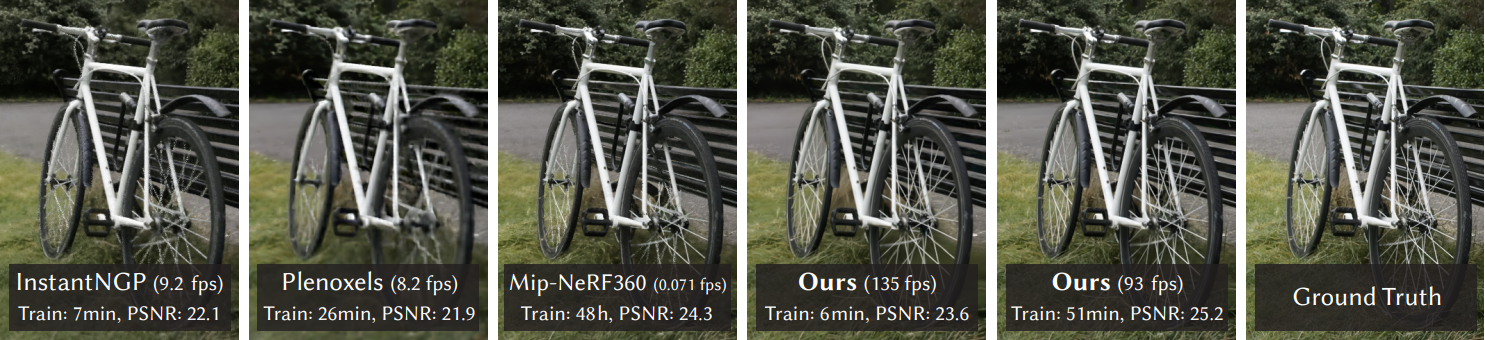
\includegraphics[width=\textwidth]{figures/3dgs_teaser.png}
  \caption{Photo-realistic novel views synthesised with 3D Gaussian Splatting at
           $>$90 fps on a consumer GPU. Each scene is reconstructed from a set of
           posed photographs; the Gaussian map supports real-time rendering from
           any viewpoint. Image from Kerbl et al.~\cite{kerbl2023gaussian}.}
  \label{fig:teaser}
\end{figure}

\medskip
The remainder of this document covers the mathematical foundations of 3DGS:
geometric representation (Sections~\ref{sec:gaussian_repr}--\ref{sec:projection}),
the rendering pipeline (Sections~\ref{sec:rasterization}--\ref{sec:alpha_blending}),
the optimisation strategy (Section~\ref{sec:optimization}), and the extension to
SLAM (Section~\ref{sec:slam}).

%==============================================================================
% Section 2 -- Mathematical Representation of 3D Gaussians
%==============================================================================
\section{Mathematical Representation of 3D Gaussians}
\label{sec:gaussian_repr}

\subsection{The 3D Gaussian Kernel}

A 3D Gaussian is defined by its unnormalised influence kernel:
\begin{equation}
  \boxed{
    \Gcal(\mathbf{x}\,;\,\mean,\cov)
    = \exp\!\left(-\frac{1}{2}(\mathbf{x}-\mean)\transp \cov^{-1} (\mathbf{x}-\mean)\right)
  }
  \label{eq:gaussian_kernel}
\end{equation}
where $\mean \in \R^3$ is the centre and $\cov \in \R^{3\times 3}$ is a
symmetric positive semi-definite (SPSD) covariance matrix. The kernel equals 1
at $\mathbf{x}=\mean$ and decays with the Mahalanobis distance; the locus
$\Gcal = e^{-1/2}$ traces the \emph{one-sigma ellipsoid}.

%------------------------------------------------------------------------------
\subsection{Gaussian Primitive}

\begin{definitionbox}{Gaussian Primitive}
Each primitive $\Gcal_i$ is an oriented, anisotropic ellipsoid characterised by:
\begin{itemize}
  \item $\mean_i \in \R^3$ -- \textbf{position},
  \item $\cov_i \in \R^{3\times 3}$ -- \textbf{shape and orientation}
        (eigenvalues = squared semi-axis lengths; eigenvectors = principal axes),
  \item $o_i \in [0,1]$ -- \textbf{opacity},
  \item $\mathbf{f}_i \in \R^{(L+1)^2 \times 3}$ -- \textbf{colour} as SH
        coefficients (Section~\ref{sec:sh}).
\end{itemize}
\end{definitionbox}

%------------------------------------------------------------------------------
\subsection{Why Gaussians?}

\begin{keybox}{Desirable Properties}
\begin{enumerate}
  \item \textbf{Differentiability}: infinitely differentiable w.r.t.\ all
        parameters, enabling gradient-based optimisation.
  \item \textbf{Closed-form projection}: a 3D Gaussian projects to a 2D
        Gaussian under a perspective camera (Section~\ref{sec:projection}).
  \item \textbf{Soft boundaries}: smooth fall-off models translucent or fuzzy
        regions (hair, smoke) without hard silhouettes.
  \item \textbf{Efficient rasterisation}: 2D splats are rendered in a single
        GPU forward pass via a tile-based rasteriser.
\end{enumerate}
\end{keybox}

%------------------------------------------------------------------------------
\subsection{Scene Representation and Parameter Count}

A scene is a finite mixture of $N$ primitives:
\begin{equation}
  \mathcal{S} = \bigl\{ (\mean_i,\, \cov_i,\, o_i,\, \mathbf{f}_i) \bigr\}_{i=1}^{N}
\end{equation}

Typical scenes contain $N \in [10^5, 10^7]$ Gaussians stored as flat GPU
tensors. For SH degree $L=3$ each Gaussian has 59 learnable parameters
($3 + 4 + 3 + 1 + 48$), so $3\times10^6$ Gaussians require $\approx700$ MB in
\texttt{float32}.

\begin{notebox}
  Directly optimising the 9 entries of $\cov$ does not guarantee SPSD. 3DGS
  instead parametrises $\cov$ through a factorisation that enforces this
  constraint by construction (Section~\ref{sec:covariance}).
\end{notebox}

%==============================================================================
% Section 3 -- Covariance Factorisation and Rotation
%==============================================================================
\section{Covariance Factorisation and Rotation}
\label{sec:covariance}

\subsection{The RS Factorisation}

To guarantee SPSD throughout optimisation, 3DGS parametrises $\cov$ as:
\begin{equation}
  \boxed{
    \cov = \rot\,\scale\,\scale\transp\rot\transp
  }
  \label{eq:cov_factorization}
\end{equation}
where $\rot \in SO(3)$ is a rotation matrix and
$\scale = \operatorname{diag}(s_1, s_2, s_3)$ with $s_k > 0$.
SPSD is guaranteed since $\mathbf{v}\transp\cov\,\mathbf{v} =
\|\scale\transp\rot\transp\mathbf{v}\|^2 \geq 0$ for all $\mathbf{v}$.
Expanded:
\begin{equation}
  \cov = \rot
  \begin{pmatrix} s_1^2 & 0 & 0 \\ 0 & s_2^2 & 0 \\ 0 & 0 & s_3^2 \end{pmatrix}
  \rot\transp
\end{equation}
The columns of $\rot$ are the eigenvectors of $\cov$ and $s_k^2$ are the
eigenvalues, so $s_k$ are the principal semi-axis lengths.

%------------------------------------------------------------------------------
\subsection{Quaternion Representation of Rotation}
\label{ssec:quaternion}

$\rot$ is stored as a unit quaternion $\quat = (q_w, q_x, q_y, q_z)$,
$\|\quat\|=1$, which uses only 4 parameters and avoids gimbal lock:
\begin{equation}
  \rot(\quat) =
  \begin{pmatrix}
    1 - 2(q_y^2 + q_z^2) & 2(q_xq_y - q_wq_z)  & 2(q_xq_z + q_wq_y) \\
    2(q_xq_y + q_wq_z)   & 1 - 2(q_x^2 + q_z^2) & 2(q_yq_z - q_wq_x) \\
    2(q_xq_z - q_wq_y)   & 2(q_yq_z + q_wq_x)   & 1 - 2(q_x^2 + q_y^2)
  \end{pmatrix}
\end{equation}
After each gradient step $\quat$ is renormalised: $\quat \leftarrow \quat/\|\quat\|$.

%------------------------------------------------------------------------------
\subsection{Scale Parametrisation}

Scales are stored as $\hat{s}_k = \log s_k \in \R$ (unconstrained) and
recovered as $s_k = \exp(\hat{s}_k)$, ensuring $s_k > 0$ without constrained
optimisation. Opacity is handled analogously via logit space.

%------------------------------------------------------------------------------
\subsection{Summary}

\begin{table}[H]
  \centering
  \caption{Learnable parameters per Gaussian primitive.}
  \label{tab:params}
  \renewcommand{\arraystretch}{1.4}
  \begin{tabular}{llll}
    \toprule
    \textbf{Attribute} & \textbf{Symbol} & \textbf{Dim.} & \textbf{Constraint} \\
    \midrule
    Position        & $\mean$               & 3          & $\R^3$ \\
    Rotation        & $\quat$               & 4          & $\|\quat\|=1$ \\
    Scale (log)     & $\hat{\mathbf{s}}$    & 3          & $\R^3$ \\
    Opacity (logit) & $\hat{o}$             & 1          & $\sigma(\hat{o})\in(0,1)$ \\
    SH coefficients & $\mathbf{f}$          & $3(L+1)^2$ & $\R$ \\
    \bottomrule
  \end{tabular}
\end{table}

%==============================================================================
% Section 4 -- Colour Modelling with Spherical Harmonics
%==============================================================================
\section{Colour Modelling via Spherical Harmonics}
\label{sec:sh}

\subsection{Motivation}

Surfaces exhibit view-dependent appearance (specular highlights, metallic
reflections). In 3DGS each Gaussian encodes its view-dependent colour compactly
using \textbf{spherical harmonics (SH)}, an orthonormal basis on the unit
sphere $S^2$

%------------------------------------------------------------------------------
\subsection{View-Dependent Colour}

For Gaussian $\Gcal_i$ and channel $k \in \{R,G,B\}$, the colour in direction
$\mathbf{d}$ is:
\begin{equation}
  \boxed{
    c_{i,k}(\mathbf{d}) = \sum_{l=0}^{L} \sum_{m=-l}^{l}
      f_{i,k,l}^m\, Y_l^m(\mathbf{d})
  }
  \label{eq:sh_color}
\end{equation}
where $f_{i,k,l}^m$ are learned coefficients. In matrix form:
$\mathbf{c}_i(\mathbf{d}) = \mathbf{F}_i\,\mathbf{y}(\mathbf{d})$,
with $\mathbf{y}(\mathbf{d}) \in \R^{(L+1)^2}$ the vector of SH values.
SH evaluation is purely polynomial, making it very efficient on the GPU.

%------------------------------------------------------------------------------
\subsection{Degree Selection}

\begin{table}[H]
  \centering
  \caption{SH parameter count by degree.}
  \label{tab:sh_count}
  \renewcommand{\arraystretch}{1.3}
  \begin{tabular}{cccc}
    \toprule
    \textbf{Max Degree $L$} & \textbf{Coeffs/channel} & \textbf{Total (RGB)} & \textbf{Effect} \\
    \midrule
    0 & 1  & 3  & Constant diffuse \\
    1 & 4  & 12 & Linear shading \\
    2 & 9  & 27 & Quadratic specular \\
    3 & 16 & 48 & Sharp specular (used in 3DGS) \\
    \bottomrule
  \end{tabular}
\end{table}

The original 3DGS paper uses $L=3$. Training starts at $L=0$ and unlocks one
degree every 1000 iterations, stabilising early optimisation by fitting
low-frequency geometry first.

\newpage

%==============================================================================
% Section 5 -- 2D Projection and EWA Splatting
%==============================================================================
\section{2D Projection and Jacobian Approximation}
\label{sec:projection}

\subsection{Overview}

Each 3D Gaussian must be projected onto the image plane. The key result is that
the projection of a 3D Gaussian under a perspective camera yields
\emph{approximately} a 2D Gaussian, following the \textbf{EWA splatting}
framework~\cite{zwicker2001ewa}.

%------------------------------------------------------------------------------
\subsection{Camera Model and Mean Projection}

A world-space point maps to camera space as
$\mathbf{x}_c = \mathbf{R}_{cw}\,\mathbf{x}_w + \mathbf{t}_{cw}$,
then projects to image coordinates:
\begin{equation}
  \pi(\mathbf{t}) =
  \begin{pmatrix} f_x\,t_x/t_z + c_x \\ f_y\,t_y/t_z + c_y \end{pmatrix}
\end{equation}
The 2D projected mean is simply $\mean'_i = \pi(\mathbf{R}_{cw}\,\mean_i +
\mathbf{t}_{cw})$.

%------------------------------------------------------------------------------
\subsection{Covariance Projection via Jacobian Approximation}

Since $\pi$ is nonlinear, a first-order Taylor expansion is used. The Jacobian
of $\pi$ at camera-space point $\mathbf{t}_i = (t_{i,x}, t_{i,y}, t_{i,z})$ is:
\begin{equation}
  \mathbf{J}_i =
  \begin{pmatrix}
    f_x/t_{i,z} & 0 & -f_x\,t_{i,x}/t_{i,z}^2 \\
    0 & f_y/t_{i,z} & -f_y\,t_{i,y}/t_{i,z}^2
  \end{pmatrix}
  \in \R^{2\times 3}
\end{equation}

The \textbf{projected 2D covariance} is:
\begin{equation}
  \boxed{
    \cov'_i = \mathbf{J}_i\,\mathbf{R}_{cw}\,\cov_i\,\mathbf{R}_{cw}\transp\,\mathbf{J}_i\transp
    \in \R^{2\times 2}
  }
  \label{eq:cov_proj}
\end{equation}

The resulting 2D splat in screen space is:
\begin{equation}
  \Gcal'_i(\mathbf{u}) =
    \exp\!\left(
      -\tfrac{1}{2}(\mathbf{u} - \mean'_i)\transp(\cov'_i)^{-1}(\mathbf{u} - \mean'_i)
    \right), \quad \mathbf{u} \in \R^2
\end{equation}
$(\cov'_i)^{-1}$ is computed in closed form since it is $2\times2$.

%------------------------------------------------------------------------------
\subsection{Bounding Box and Tile Culling}

For each splat, a bounding box of half-extent $r = 3\sqrt{\lambda_{\max}(\cov'_i)}$
(the $3\sigma$ ellipse, capturing $>99\%$ of the Gaussian's mass) determines
which screen tiles overlap with the splat. Pixels outside this radius are
discarded, reducing per-tile Gaussian counts significantly.

The Jacobian-based approach is chosen because it is accurate for typical scene
scales and fully differentiable, enabling gradient flow through the projection.

%==============================================================================
% Section 6 -- Differentiable Rasterisation Pipeline and Tiling
%==============================================================================
\section{Differentiable Rasterisation Pipeline and Tiling}
\label{sec:rasterization}

\subsection{Design Goals}

The pipeline must be: (1) \textbf{real-time} ($<$10 ms/frame at 1080p),
(2) \textbf{differentiable} (gradients back to all Gaussian parameters), and
(3) \textbf{depth-correct} (front-to-back compositing). These are achieved
via a \textbf{tile-based, sorting-based CUDA rasteriser}.

%------------------------------------------------------------------------------
\subsection{Pipeline Overview}

\begin{algorithm}[H]
  \caption{3DGS Differentiable Rasterisation Pipeline}
  \label{alg:pipeline}
  \begin{algorithmic}[1]
    \Require{Gaussian set $\mathcal{S}$, camera parameters, resolution $W \times H$}
    \Ensure{Rendered image $\hat{I}$}
    \State \textbf{Preprocessing} (parallel over all $N$ Gaussians):
      project means, compute 2D covariances, evaluate SH colours, compute
      bounding boxes and depths.
    \State \textbf{Tile assignment}: divide screen into $16\times16$ tiles;
      for each Gaussian, append a 64-bit key
      $[\tau\texttt{\_id}\,\|\,z_i]$ for every overlapping tile.
    \State \textbf{GPU radix sort} by key $\Rightarrow$ depth order per tile
      ($O(M)$, $\sim10^9$ keys/s).
    \For{each tile $\tau$ \textbf{in parallel} (one CUDA block)}
      \For{each pixel $\mathbf{u}$ in $\tau$}
        \State Accumulate colour via alpha blending
               (Algorithm~\ref{alg:alpha_blend}).
      \EndFor
    \EndFor
    \State \Return{$\hat{I}$}
  \end{algorithmic}
\end{algorithm}

%------------------------------------------------------------------------------
\subsection{Tile Decomposition}

The screen is split into $16\times16$ pixel tiles (256 threads/block, a
multiple of the CUDA warp size). Pixels in the same tile share most Gaussians,
enabling cooperative shared-memory loading.

%------------------------------------------------------------------------------
\subsection{CUDA Rendering and Early Termination}

Each CUDA block loads batches of 128 Gaussians into shared memory and each
thread accumulates its pixel colour independently. A thread maintains
accumulated transmittance $T$; when $T < \epsilon = 10^{-4}$ the pixel is
\emph{saturated} and the thread exits, providing significant speed-ups for
occluded pixels.

%------------------------------------------------------------------------------
\subsection{Backward Pass}

A custom CUDA kernel re-traces the forward pass in \emph{reverse tile order}
(back-to-front), accumulating gradients
$\partial\mathcal{L}/\partial\mean'_i$,
$\partial\mathcal{L}/\partial\cov'_i$,
$\partial\mathcal{L}/\partial o_i$,
$\partial\mathcal{L}/\partial\mathbf{c}_i$
via atomic operations. World-space gradients are then obtained by autodiff
through the preprocessing pass. The overall pipeline scales as $O(N)$ in
Gaussians and $O(WH)$ in pixels.

%==============================================================================
% Section 7 -- Alpha Blending and Accumulation Rendering
%==============================================================================
\section{Alpha Blending and Accumulation Rendering}
\label{sec:alpha_blending}

\subsection{Alpha Compositing}

Given $N$ colour contributions $\{c_i\}$ with opacities $\{\alpha_i\}$ sorted
front-to-back, the final pixel colour is:
\begin{equation}
  \boxed{
    C = \sum_{i=1}^{N} c_i\,\alpha_i\,T_i
  }, \qquad
  T_i = \prod_{j=1}^{i-1}(1 - \alpha_j), \quad T_1 = 1
  \label{eq:alpha_blend}
\end{equation}
$T_i$ is the transmittance reaching layer $i$; $\alpha_i T_i$ is its effective
contribution.

%------------------------------------------------------------------------------
\subsection{Per-Gaussian Opacity at a Pixel}

The opacity of Gaussian $\Gcal_i$ at pixel $\mathbf{u}$ combines the learned
opacity $o_i$ and the 2D kernel response:
\begin{equation}
  \boxed{
    \alpha_i(\mathbf{u}) = o_i \cdot
      \exp\!\left(
        -\tfrac{1}{2}(\mathbf{u} - \mean'_i)\transp(\cov'_i)^{-1}(\mathbf{u} - \mean'_i)
      \right)
  }
  \label{eq:per_gaussian_alpha}
\end{equation}

%------------------------------------------------------------------------------
\subsection{Incremental Accumulation}

\begin{algorithm}[H]
  \caption{Alpha Blending per Pixel (front-to-back)}
  \label{alg:alpha_blend}
  \begin{algorithmic}[1]
    \Require{Sorted Gaussians $\{i_1, \ldots, i_K\}$ covering pixel $\mathbf{u}$}
    \Ensure{Pixel colour $C(\mathbf{u})$}
    \State $C \leftarrow \mathbf{0}$, \quad $T \leftarrow 1$
    \For{$k = 1, \ldots, K$}
      \State $\alpha \leftarrow \alpha_{i_k}(\mathbf{u})$
      \If{$\alpha < \epsilon_{\min}$} \textbf{continue} \EndIf
      \State $C \leftarrow C + \mathbf{c}_{i_k} \cdot \alpha \cdot T$; \quad
             $T \leftarrow T \cdot (1 - \alpha)$
      \If{$T < \epsilon_{\text{stop}}$} \textbf{break} \EndIf
    \EndFor
    \State \Return{$C + T \cdot C_{\text{bg}}$}
  \end{algorithmic}
\end{algorithm}

$\epsilon_{\min} = \epsilon_{\text{stop}} = 10^{-4}$. Depth and opacity maps
are obtained by the same accumulation replacing $\mathbf{c}_i$ with $z_i$ or 1:
\begin{equation}
  D(\mathbf{u}) = \sum_i z_i\,\alpha_i\,T_i, \qquad
  A(\mathbf{u}) = 1 - T_{\text{final}}
\end{equation}

%------------------------------------------------------------------------------
\subsection{Connection to NeRF Volume Rendering}

The 3DGS formula is the discrete equivalent of the NeRF volume integral.
Identifying $\alpha_i = 1 - e^{-\sigma_i\delta_i}$ and
$T_i = \prod_{j<i}e^{-\sigma_j\delta_j}$ recovers Eq.~\eqref{eq:alpha_blend}
exactly. The two methods differ only in \emph{how} $\alpha_i$ is produced, not
in the compositing formula.

%==============================================================================
% Section 8 -- Optimisation: Densification, Pruning, and Opacity
%==============================================================================
\section{Optimisation Mechanisms: Densification, Pruning, and Opacity}
\label{sec:optimization}

\subsection{Training Objective}

All parameters are optimised end-to-end by minimising:
\begin{equation}
  \boxed{
    \mathcal{L} = (1 - \lambda)\,\mathcal{L}_1 + \lambda\,\mathcal{L}_{\text{D-SSIM}}
  }, \quad \lambda = 0.2
\end{equation}
$\mathcal{L}_1$ ensures per-pixel accuracy; $\mathcal{L}_{\text{D-SSIM}}$
preserves structural detail by penalising blurry renderings.

%------------------------------------------------------------------------------
\subsection{Optimiser}

Adam with per-group learning rates (position: $1.6\times10^{-4}$ decaying to
$1.6\times10^{-6}$; scale: $5\times10^{-3}$; rotation: $10^{-3}$; opacity:
$5\times10^{-2}$; SH degree 0: $2.5\times10^{-3}$; SH 1--3:
$2.5\times10^{-4}$).

%------------------------------------------------------------------------------
\subsection{Adaptive Density Control}
\label{ssec:density}

Every 100 iterations (from iter.\ 500 to 15\,000), the mean position gradient
\begin{equation}
  \bar{\nabla}_i = \tfrac{1}{K}\sum_{k=1}^{K}\|\nabla_{\mean'_i}\mathcal{L}\|
\end{equation}
drives two operations when $\bar{\nabla}_i > \tau_{\text{grad}} = 2\times10^{-4}$:

\begin{itemize}
  \item \textbf{Clone} (small Gaussian, $\max s_k < \tau_{\text{size}}$): create
        an exact copy; both are optimised independently. The region needs more
        primitives.
  \item \textbf{Split} (large Gaussian, $\max s_k \geq \tau_{\text{size}}$):
        replace with two Gaussians at scale $s_k/1.6$, positions sampled from
        $\mathcal{N}(\mean_i, \cov_i)$. The primitive covers too large an area.
\end{itemize}

%------------------------------------------------------------------------------
\subsection{Pruning}

At the same frequency, Gaussians are removed if: (1) opacity
$o_i < \epsilon_\alpha = 0.005$, (2) world-space size exceeds $\tau_w$, or
(3) projected 2D radius exceeds $\tau_v$ (removes ``floaters'').

%------------------------------------------------------------------------------
\subsection{Periodic Opacity Reset}

Every 3000 iterations all opacities are reset to $\alpha_{\min} \approx 0.01$.
Gaussians that contribute to the scene recover high opacity quickly; redundant
ones do not and are pruned at the next pruning step. This prevents ghost
Gaussians from accumulating throughout training.

%------------------------------------------------------------------------------
\subsection{Training Schedule and Convergence}

\begin{algorithm}[H]
  \caption{3DGS Training Schedule (30\,000 iterations)}
  \label{alg:training}
  \begin{algorithmic}[1]
    \Require{Images $\{I_k\}$, SfM point cloud $\mathcal{P}$}
    \State Initialise small isotropic Gaussians from $\mathcal{P}$
    \For{$t = 1, \ldots, 30000$}
      \State Render $\hat{I}$; compute $\mathcal{L}$; Adam step
      \If{$500 \leq t \leq 15000$ and $t \bmod 100 = 0$}
        \State Clone/split high-gradient Gaussians; prune low-opacity/large ones
      \EndIf
      \If{$t \bmod 3000 = 0$} Reset opacities to $\alpha_{\min}$ \EndIf
      \If{$t \bmod 1000 = 0$ and $t \leq 3000$} Unlock next SH degree \EndIf
    \EndFor
  \end{algorithmic}
\end{algorithm}

A typical run starts with $\sim10^4$--$10^5$ Gaussians, peaks at
$\sim3\times10^6$--$6\times10^6$, and stabilises at
$\sim10^6$--$4\times10^6$. Training takes 20--45 min on an RTX 3090/4090;
at convergence rendering exceeds 90 fps at $1920\times1080$.

%==============================================================================
% Section 9 -- 3DGS for SLAM
%==============================================================================
\section{3D Gaussian Splatting for SLAM}
\label{sec:slam}

\subsection{Simultaneous Localisation and Mapping}

Simultaneous Localisation and Mapping (SLAM) addresses the chicken-and-egg
problem of robotic perception: a moving agent must estimate its own pose
(localisation) while concurrently building a map of the environment (mapping),
without prior knowledge of either.  Classical SLAM pipelines rely on sparse or
semi-dense geometric representations such as point clouds, occupancy grids, and
keyframe-based pose graphs.  These representations are efficient but lack visual
fidelity, making them unsuitable for applications that require photorealistic
reconstructions, such as augmented reality or human-robot interaction.

3DGS offers a compelling alternative: the same Gaussian primitives used for
novel-view synthesis can serve as the scene map, providing simultaneously a
dense, photorealistic, and differentiable representation that can be queried or
rendered in real time.

%------------------------------------------------------------------------------
\subsection{Integration of 3DGS into the SLAM Pipeline}

A 3DGS-SLAM system alternates between two tightly coupled phases:

\begin{enumerate}
  \item \textbf{Tracking.}  Given the current Gaussian map, the camera pose
        $T_t \in SE(3)$ is estimated by minimising a photometric loss between
        the rendered frame (obtained by splatting the existing Gaussians from
        the candidate pose) and the actual camera observation:
        \begin{equation}
          T_t^* = \arg\min_{T_t} \sum_{p} \bigl\|
            \hat{I}(p;\,T_t,\,\mathcal{G}) - I_t(p)
          \bigr\|_1,
          \label{eq:slam_tracking}
        \end{equation}
        where $\hat{I}(p;\,T_t,\,\mathcal{G})$ is the rendered colour at pixel
        $p$ given map $\mathcal{G}$ and pose $T_t$, and $I_t$ is the observed
        frame.

  \item \textbf{Mapping.}  Once the pose is fixed, the Gaussian map is updated
        by (a) spawning new Gaussians at the depth of pixels with high
        photometric error, and (b) optimising all Gaussian parameters via
        back-propagation through the differentiable renderer, exactly as in
        the offline 3DGS pipeline (Section~\ref{sec:optimization}).
\end{enumerate}

\begin{figure}[H]
  \centering
  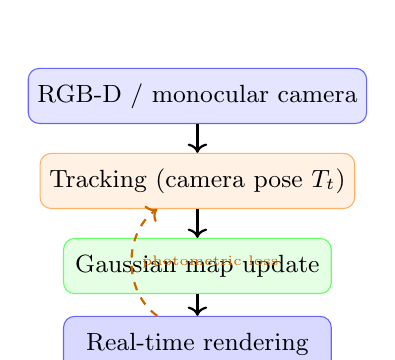
\begin{tikzpicture}[scale=0.9, every node/.style={font=\small},
      box/.style={draw, rounded corners, minimum width=3.4cm,
                  minimum height=0.7cm, align=center}]
    \node[box, fill=blue!10,   draw=blue!60]   (cam)   at (0,3.5) {RGB-D / monocular camera};
    \node[box, fill=orange!10, draw=orange!60] (track) at (0,2.3) {Tracking (camera pose $T_t$)};
    \node[box, fill=green!10,  draw=green!60]  (map)   at (0,1.1) {Gaussian map update};
    \node[box, fill=blue!15,   draw=blue!60]   (ren)   at (0,0.0) {Real-time rendering};
    \draw[->, thick] (cam)   -- (track);
    \draw[->, thick] (track) -- (map);
    \draw[->, thick] (map)   -- (ren);
    \draw[->, thick, dashed, orange!80!black] (ren)
      to[bend left=55] node[right, font=\tiny] {photometric loss}  (track);
  \end{tikzpicture}
  \caption{Data-flow in a 3DGS-SLAM system.  Tracking and mapping alternate
           at each keyframe; the differentiable renderer couples both phases.}
  \label{fig:slam_pipeline}
\end{figure}

%------------------------------------------------------------------------------
\subsection{Notable 3DGS-SLAM Systems}

\begin{table}[H]
  \centering
  \caption{Comparison of published 3DGS-SLAM methods.}
  \label{tab:slam_systems}
  \renewcommand{\arraystretch}{1.4}
  \begin{tabular}{l p{3.2cm} p{4.0cm} p{3.5cm}}
    \toprule
    \textbf{System} & \textbf{Input} & \textbf{Key contribution} & \textbf{Speed} \\
    \midrule
    SplaTAM~\cite{keetha2024splatam} &
      RGB-D &
      Silhouette-guided densification; first real-time 3DGS SLAM &
      $\sim$10 fps mapping \\
    Gaussian-SLAM &
      RGB-D &
      Online reconstruction with sub-map merging &
      $>$10 fps on one GPU \\
    MonoGaussian &
      Monocular RGB &
      Depth estimated from monocular cues; no depth sensor &
      Real-time capable \\
    \bottomrule
  \end{tabular}
\end{table}

%------------------------------------------------------------------------------
\subsection{Advantages and Open Challenges}

\paragraph{Advantages over classical SLAM representations.}
\begin{itemize}
  \item \textbf{Photorealism.}  The Gaussian map supports novel-view rendering,
        enabling downstream tasks such as loop closure via appearance-based
        place recognition.
  \item \textbf{Differentiability.}  Pose optimisation is formulated as gradient
        descent through the renderer (Eq.~\ref{eq:slam_tracking}), without
        requiring hand-crafted feature descriptors.
  \item \textbf{Real-time rendering.}  The GPU-rasterised pipeline delivers
        $>$90 fps renders even during online mapping.
\end{itemize}

\paragraph{Open challenges.}
\begin{itemize}
  \item \textbf{Memory growth.}  The number of Gaussians grows with scene size,
        making large-scale outdoor SLAM memory-intensive.
  \item \textbf{Loop closure.}  Correcting accumulated drift requires updating
        potentially millions of Gaussians consistently.
  \item \textbf{Dynamic objects.}  Moving people or vehicles violate the static
        scene assumption and produce rendering artefacts.
  \item \textbf{Monocular scale ambiguity.}  Without depth, metric scale must
        be recovered from additional cues or a known object.
\end{itemize}

\begin{keybox}{Summary}
  3DGS-SLAM unifies photorealistic scene reconstruction and real-time
  camera tracking in a single differentiable framework, combining the
  speed of GPU rasterisation with the accuracy of gradient-based pose
  optimisation.  Current systems achieve real-time performance on RGB-D
  input; extending them to monocular and large-scale outdoor settings
  remains an active research area.
\end{keybox}

%==============================================================================
% Section 12 -- Uncertainty and Initialization
%==============================================================================
\section{Uncertainty Management and Point Initialization}
\label{sec:point_init}

The transition from 2D observations to 3D Gaussian primitives requires robust initialization and filtering to maintain map integrity.

\paragraph{Depth-Based Seeding.} 
In RGB-D configurations, the initial position $\mu$ of a Gaussian is back-projected from the depth map $D_t$. The initial scale $s$ is typically set to:
\begin{equation}
    s_{init} = \lambda \cdot \frac{D_t(p)}{f},
\end{equation}
where $f$ is the focal length and $\lambda$ is a scaling factor to ensure initial coverage.

\paragraph{Pruning and Densification.} 
Uncertainty is managed through a "survive-of-the-fittest" approach. Gaussians are pruned if their opacity $\alpha$ falls below a threshold $\epsilon_{\alpha}$ or if their view-space position exhibits high variance over multiple frames. Conversely, in regions where the rendered silhouette $S(p)$ is near zero but an observation exists, new Gaussians are spawned to fill "holes" in the geometry.
%==============================================================================
% Section 12 -- Uncertainty and Initialization
%==============================================================================
\section{Loop Closure and Global Optimization}
\label{sec:opti}

%------------------------------------------------------------------------------
As the camera traverses large environments, small errors in pose estimation (Eq.~\ref{eq:slam_tracking}) accumulate, leading to "drift" where the reconstructed map no longer aligns with reality upon revisiting a known location.
\paragraph{Place Recognition.}
Loop closure detection in 3DGS-SLAM typically leverages the photorealistic nature of the map. Systems compare the current live frame $I_t$ against a database of previous keyframes using global image descriptors (e.g., NetVLAD or DBoW2). If a high-similarity match is found, a loop candidate is identified.
\paragraph{Global Bundle Adjustment (GBA).}
Once a loop is detected, the system must perform a global correction. Unlike traditional SLAM, which only optimizes a pose graph, 3DGS-SLAM must adjust:
\begin{itemize}
    \item \textbf{Camera Poses:} Correcting the historical trajectory to close the geometric gap. 
    \item \textbf{Gaussian Parameters:} Aligning the primitives $\{\mu_i, \Sigma_i\}$ to the new optimized poses. 
\end{itemize}
\paragraph{Sub-map Merging.}
Advanced systems like \textit{Gaussian-SLAM} manage large-scale scenes by dividing the environment into independent sub-maps. When a loop is closed, these sub-maps are merged by performing a rigid transformation on the Gaussian collections to ensure seamless visual and geometric transitions.
%==============================================================================
% Section 14 -- Performance Analysis
%==============================================================================
\section{Performance Analysis: Latency, FPS, and VRAM Consumption}
\label{sec:analysis}

The fundamental architectural differences between NeRF (implicit, continuous) and 3DGS (explicit, discrete) manifest most prominently in their hardware utilization during SLAM operations. The choice between the two paradigms generally represents a trade-off between computational latency and memory consumption.

\subsection{Computational Latency and FPS}
NeRF-based SLAM systems, such as iMAP and NICE-SLAM, rely on volumetric ray marching. To render a single pixel for photometric loss calculation, the system must query a Multi-Layer Perceptron (MLP) or feature grid hundreds of times along a camera ray. This heavy computational burden restricts tracking and mapping speeds to typically $1$--$5$ Frames Per Second (FPS), and makes real-time novel view rendering ($>30$ FPS) nearly impossible without specialized hardware.

In contrast, 3DGS-SLAM systems (e.g., SplaTAM~\cite{keetha2024splatam}, Gaussian-SLAM) bypass ray marching in favor of tile-based rasterization. Because projecting 3D ellipsoids onto a 2D plane is a highly parallelizable and native GPU operation, tracking and mapping can be performed at $10$--$30$ FPS. Furthermore, the decoupling of the mapping thread from the rendering thread allows 3DGS-SLAM to render the live reconstructed scene at $>90$ FPS, making it vastly superior for real-time AR/VR applications.

\subsection{VRAM Consumption and Scalability}
While 3DGS excels in compute speed, it suffers from a severe memory bottleneck. NeRFs encode the scene implicitly; the entire geometry and appearance of a room can be compressed into the weights of an MLP and a multi-resolution hash grid, often consuming less than $1$ GB of Video RAM (VRAM).

Conversely, 3DGS requires explicit storage for every primitive. Each 3D Gaussian must store its position $\mu \in \mathbb{R}^3$, covariance matrix components (scale $s \in \mathbb{R}^3$ and rotation quaternion $q \in \mathbb{R}^4$), opacity $\alpha \in \mathbb{R}$, and Spherical Harmonic (SH) coefficients for view-dependent color. 
A single high-fidelity indoor room can easily require $1$ to $3$ million Gaussians, consuming $2$--$6$ GB of VRAM. In large-scale trajectory mapping without aggressive pruning, the Gaussian count can explode, pushing VRAM consumption beyond $24$ GB and severely limiting the deployment of 3DGS-SLAM on resource-constrained embedded systems or mobile robots.

\begin{table}[H]
  \centering
  \caption{Empirical Performance Trade-offs in Real-Time SLAM}
  \label{tab:performance_comparison}
  \renewcommand{\arraystretch}{1.4}
  \begin{tabular}{l p{3.5cm} p{3.5cm}}
    \toprule
    \textbf{Metric} & \textbf{NeRF-SLAM} & \textbf{3DGS-SLAM} \\
    \midrule
    \textbf{Tracking \& Mapping Speed} & $1$ -- $5$ FPS & $10$ -- $30+$ FPS \\
    \textbf{Rendering Speed} & $< 10$ FPS & $> 90$ FPS \\
    \textbf{VRAM Footprint (Room Scale)} & $< 1$ GB & $2$ -- $6$ GB \\
    \textbf{Primary Bottleneck} & Computational \newline (Compute Bound) & Memory \newline (Memory Bound) \\
    \textbf{Mobile Suitability} & Moderate \newline (High Latency) & Poor \newline (High VRAM) \\
    \bottomrule
  \end{tabular}
\end{table}

%------------------------------------------------------------------------------
\subsection{SLAM Evaluation Metrics}

To rigorously compare the performance of NeRF-based and 3DGS-SLAM systems, evaluations are typically divided into two distinct categories: tracking accuracy (localisation) and mapping fidelity (reconstruction).

\paragraph{Tracking Accuracy.} 
The precision of the estimated camera trajectory is evaluated against a known ground-truth trajectory using the \textbf{Absolute Trajectory Error (ATE)}. The ATE measures the global consistency of the estimated trajectory by first aligning it to the ground truth (usually via Horn's method) and then computing the Root Mean Square Error (RMSE) of the translational differences. Mathematically, for an estimated trajectory $T$ and ground truth $Q$, the ATE RMSE over $N$ frames is defined as:
\begin{equation}
    \text{ATE}_{\text{RMSE}} = \left( \frac{1}{N} \sum_{i=1}^{N} \bigl\| \text{trans}(Q_i^{-1} S T_i) \bigr\|^2 \right)^{1/2}
\end{equation}
where $S$ is the rigid alignment transformation.

\paragraph{Mapping and Rendering Quality.} 
Because both NeRF and 3DGS are inherently view-synthesis formulations, the quality of the reconstructed map is evaluated by freezing the map, rendering novel views from held-out ground-truth poses, and comparing the results to the actual captured images. The standard photometric metrics include:
\begin{itemize}
    \item \textbf{PSNR (Peak Signal-to-Noise Ratio):} Measures pixel-wise accuracy. Higher is better.
    \item \textbf{SSIM (Structural Similarity Index):} Measures perceived changes in structural information, capturing high-frequency details. Higher is better (maximum is 1.0).
    \item \textbf{LPIPS (Learned Perceptual Image Patch Similarity):} Evaluates deep-feature differences using a pre-trained network (like VGG), providing a metric that closely aligns with human visual perception. Lower is better.
\end{itemize}

While NeRF and 3DGS systems often achieve comparable ATE RMSE (typically in the range of $1$ to $5$ cm on standard datasets like Replica or TUM-RGBD), 3DGS systems generally edge out NeRFs in mapping metrics (PSNR, SSIM) due to the explicit representation preserving sharp high-frequency details better than continuous MLPs.
%==============================================================================
% Section 14 -- Limitations
%==============================================================================
\section{Limitations: Dynamic Scenes, Compression, and Storage}
\label{sec:limitations}

Despite the real-time rendering and tracking advantages of 3DGS over NeRF, the explicit nature of Gaussian splatting introduces unique limitations regarding scene dynamics and long-term data storage.

\paragraph{Handling Dynamic Scenes.} 
Standard 3DGS-SLAM relies on a strict static-world assumption. When moving objects (e.g., pedestrians, vehicles, or moving shadows) enter the camera's view, the tracking thread registers high photometric error. The mapping thread responds by improperly spawning "floater" Gaussians in mid-air to satisfy the momentary view, resulting in persistent ghosting artefacts in the final map. 
While some NeRF-SLAM systems handle dynamics by learning transient density fields, 3DGS must adopt explicit temporal modelling. Recent extensions, such as \textit{4D Gaussian Splatting (4DGS)} or \textit{Dynamic 3DGS}, address this by attaching a time-dependent velocity vector or a learned deformation field to each Gaussian primitive. However, integrating these 4D representations into a real-time SLAM pipeline remains computationally prohibitive and is an active area of research.

\paragraph{Persistent Storage and Compression.} 
While Section~\ref{sec:analysis}.2 discussed the runtime Video RAM (VRAM) bottleneck, the persistent storage (disk space) required to save a reconstructed Gaussian map is equally problematic. NeRF models can compress an entire scene into a few megabytes of neural network weights. In contrast, saving a 3DGS map involves serializing millions of primitives. A standard 3 million Gaussian scene requires approximately $700$ MB to $1$ GB of disk space in \texttt{float32} precision.

To mitigate this, recent literature has proposed aggressive compression techniques for explicit volumetric representations:
\begin{itemize}
    \item \textbf{Vector Quantization (VQ):} Instead of storing unique Spherical Harmonic (SH) coefficients and covariance matrices for every Gaussian, primitives are clustered into a smaller "codebook" of shared properties.
    \item \textbf{Attribute Pruning:} The highest-order SH bands (degrees $L=2$ and $L=3$) consume the vast majority of parameters. Selectively dropping these bands for Gaussians in textureless regions drastically reduces the file size without degrading perceived quality.
    \item \textbf{Entropy Coding:} Sorting Gaussians spatially (e.g., via Morton coding) and applying standard lossless compression algorithms can reduce the storage footprint by over $50\%$, bringing the storage requirements closer to practical limits for mobile robotics.
\end{itemize}
%==============================================================================
% Section 15 -- Conclusion
%==============================================================================
\section{Conclusions and Future Directions}
\label{sec:conclusion}

En este estudio comparativo, hemos analizado los fundamentos matemáticos y la integración en sistemas SLAM de 
3D Gaussian Splatting (3DGS)~\cite{kerbl20233d} frente a Neural Radiance Fields (NeRF)~\cite{mildenhall2020nerf}. 
La transición de representaciones implícitas y continuas (NeRF) a representaciones explícitas y discretas (3DGS) 
marca un cambio de paradigma fundamental en los sistemas de percepción robótica, 
trasladando el principal cuello de botella del hardware desde la capacidad de cómputo hacia el consumo de memoria.

Por un lado, 3DGS ha demostrado ser abrumadoramente superior en términos de latencia y velocidad computacional. 
Al reemplazar el costoso proceso de \textit{ray marching} volumétrico de NeRF por una rasterización de primitivas 
explícitas acelerada por GPU, 3DGS logra velocidades de seguimiento y mapeo de 10 a más de 30 
FPS~\cite{keetha2024splatam}, junto con un renderizado fotorrealista en tiempo real que supera los 90 FPS. 
Además, su representación geométrica explícita preserva mejor los detalles de alta frecuencia en las métricas 
de evaluación de mapas (como PSNR y SSIM). Estas características hacen de 3DGS la tecnología idónea para 
aplicaciones interactivas como la realidad aumentada y virtual (AR/VR).

Sin embargo, estas ventajas conllevan compromisos críticos. La naturaleza explícita de 3DGS sufre de un severo 
consumo de memoria de video (VRAM) y espacio de almacenamiento persistente. Mientras que NeRF puede comprimir la
 información de una escena entera en menos de 1 GB de VRAM gracias a los pesos de su red neuronal, 
 3DGS requiere instanciar millones de elipsoides, pudiendo sobrepasar rápidamente los 24 GB en mapeos de 
 trayectorias a gran escala. Adicionalmente, la dependencia de 3DGS de un entorno estrictamente estático hace 
 que la presencia de objetos dinámicos genere artefactos visuales, requiriendo el uso de complejas extensiones 
 temporales como 4DGS que hoy en día resultan computacionalmente prohibitivas.

En resumen, 3DGS-SLAM unifica la reconstrucción fotorrealista de alta fidelidad y el seguimiento de cámaras en 
tiempo real, superando las barreras de latencia de las arquitecturas NeRF. El éxito y la adopción futura de 3DGS 
en plataformas con recursos limitados (como robots móviles o sistemas integrados) dependerán de la investigación 
activa en técnicas agresivas de compresión, como la cuantización vectorial, la poda de atributos y la codificación
de entropía, así como de un modelado eficiente para escenas dinámicas.

%==============================================================================
% Bibliography
%==============================================================================
\newpage
\bibliographystyle{plain}
\bibliography{references}

\end{document}
